\documentclass{article}
\author{Oscar Wu}
\date{}
\title{Reference Report}
\usepackage[margin=1 in]{geometry}
\usepackage{url}
\usepackage{hyperref}
\usepackage{graphicx}


\begin{document}
\bf{\maketitle}

\section{Introduction}
This report is for Prof Gleb referencing codes in repository: 
\begin{center}
\href{https://github.com/wuyoscar/MOOP}{GitHub}   
\end{center}

\noindent Most of codes based on package \emph{pymoo}. Reason of using this package to working this project show the table below:
\begin{table}[h]
	\caption{Multi-objective Optimization Frameworks in Python}
		\begin{center}
			\begin{tabular}{|c|c|c|c|c|}
			\hline 
			Name & Focus on multi-objective & Pure python &Visualization & Decision Making \\
			\hline 
			jMetalPy & $\surd$ & $\surd$ & $\surd$  & $\times $  \\
            \hline 
			PyGMO & $\surd$ & $\times$ & $\times$  & $\times $  \\
            \hline 
			Platypus & $\surd$ & $\surd$ & $\times$  & $\times $  \\
            \hline 
			DEAP & $\times$ & $\surd$ & $\times$  & $\times $  \\
            \hline 
			Inspyred & $\times$ & $\surd$ & $\times$  & $\times $  \\
            \hline 
			\bf{pymoo} & $\surd$ & $\surd$ & $\surd$  & $\surd $  \\

            \hline
			\end{tabular}
		\end{center}
	\end{table}
\section{Architecture}
\begin{description}
    \item[\bf{Probelms:}]
    Optimization problems in framework
    are categorized into single, multi, and many-objective
    test problems. Gradients are available through automatic
    differentiation and parallelization can be implemented
    by using a variety of techniques \cite{Blank2020}.
    \item[Optimization:] Most of the algorithms are based
    on evolutionary computations \cite{Blank2020}, operators such as sampling, mating selection, crossover and mutation have to
    be chosen or implemented. Moreover, when the algorithm is
    used to solve the problem, a termination criterion must
    be defined either explicitly or implicitly by the implementation of the algorithm.
    \item[Analytics:]  During and after an optimization run analytics support the understanding of data\cite{Blank2020}. First, intuitively the design space, objective space, or other metrics can be explored through visualization. Moreover, to
    measure the convergence and/or diversity of a Pareto optimal set performance indicators can be used.
\end{description}

\section{Problems}
\subsection{Problem Table}

\begin{table}[h]
\caption{Problem table}  
\begin{center}
\begin{tabular}{|c||c|c|c|}
    \hline
    \multicolumn{4}{|c|}{\bf{Problems List}} \\
    \hline
    Problem Name     & \# Variables & \# Objectives &\# Constraints\\
    \hline
    \href{https://en.wikipedia.org/wiki/Test_functions_for_optimization}{Binh and Korn function}   & 2    &2&   2\\
    \hline
    \href{https://pymoo.org/problems/multi/bnh.html}{BNH} &2 & 2& 2\\
    \hline
    \href{https://en.wikipedia.org/wiki/Test_functions_for_optimization}{Chankong and Hamies function}&   2  & 2   &2\\
    \hline
    \href{https://en.wikipedia.org/wiki/Test_functions_for_optimization}{Constr-Ex problem} &2 & 2&  2\\
    \hline
    \href{https://pymoo.org/problems/multi/osy.html}{OSY} &6&2&6 \\
    \hline
    \href{https://pymoo.org/problems/multi/truss2d.html}{Truss2D} &3&2&1\\
    \hline
    \href{https://pymoo.org/problems/multi/welded_beam.html}{Welded beam} &4&2&4\\

    \hline
    \href{https://pymoo.org/problems/multi/zdt.html#ZDT1}{zdt1} &30&30&None \\
    \hline
    \href{https://pymoo.org/problems/multi/zdt.html#ZDT2}{zdt2} &30 &2&None \\
    \hline
    \href{https://pymoo.org/problems/multi/zdt.html#ZDT3}{zdt3} &30&2&None \\
    \hline
    \href{https://pymoo.org/problems/multi/zdt.html#ZDT4}{zdt4} &10&2&None \\
    \hline
    \href{https://pymoo.org/problems/multi/zdt.html#ZDT5}{zdt5} &80&2&None \\
    \hline
    \href{https://pymoo.org/problems/constrained/dascmop.html}{DASCMOP1} &30&2&11\\
    \hline
    
\end{tabular}
\end{center}
\label{table:problem}
\end{table}

Table~\ref*{table:problem} shows the problems list. Clicking the problem name to access formula webpage. The first four problems, from \emph{``Binh and Korn function''}
to \emph{``Constr-Ex problem''} define by users. The rest of problems can be called from \emph{pymoo} package. There are other available problems in package (\href{https://pymoo.org/problems/index.html}{Other availabel problems}). 

\subsection{Problems Codes}
The location of problems code is here  \href{https://github.com/wuyoscar/MOOP/tree/master/Loopfiles/problems}{Repository}.
\begin{enumerate}
    \item Only need users to give the input range (Random search). 
    \item Then run the python problem script 
    \item The script will generate four files: a)Feasible X, b)Feasible objective value, c)Infeasible X, d)Infeasible objective value.
\end{enumerate}

\subsection{Outcome of problem files}
Purpose of problems files is given random input, splitting input into feasible and infeasible, and visualizing the output (Visualization deleted in loop files). Because in pymoo package, algorithms files only outputs best objective function value. 
In other words, algorithm only return the non-dominated set of solution.  

\section{Algorithm}
\subsection{Algorithm Table}
\begin{table}[h]
    \caption{Algorithm table}  
    \begin{center}
    \begin{tabular}{|c|c|}
        \hline
        \multicolumn{2}{|c|}{\bf{Algorithm List}} \\
        \hline
        Algorithm Name     & \# Parameter\\

        \hline
        NSGAII & \href{https://github.com/wuyoscar/MOOP/blob/master/Loopfiles/algorithmns/NSGA-II/NSGA-II_crossover.py}{crossover}, \href{https://github.com/wuyoscar/MOOP/blob/master/Loopfiles/algorithmns/NSGA-II/NSGA-II_evals.py}{\#evaluzations}, 
        \href{https://github.com/wuyoscar/MOOP/blob/master/Loopfiles/algorithmns/NSGA-II/NSGA-II_generation.py}{\#generate},
        \href{https://github.com/wuyoscar/MOOP/blob/master/Loopfiles/algorithmns/NSGA-II/NSGA-II_mutation.py}{Mutation},
        \href{https://github.com/wuyoscar/MOOP/blob/master/Loopfiles/algorithmns/NSGA-II/NSGA-II_popsize.py}{Population}\\
        \hline
        RNSGA-II & \href{https://github.com/wuyoscar/MOOP/blob/master/Loopfiles/algorithmns/RNSGA-II/RNSGA-II_episilon.py}{Episilon}, \href{https://github.com/wuyoscar/MOOP/blob/master/Loopfiles/algorithmns/RNSGA-II/RNSGA-II_refer_points.py}{Refer\_point},\href{https://github.com/wuyoscar/MOOP/blob/master/Loopfiles/algorithmns/RNSGA-II/RNSGA-II_weight.py}{Weight}  \\ 
        \hline
        NSGAIII & \href{https://github.com/wuyoscar/MOOP/blob/master/Loopfiles/algorithmns/NSGA-III/NSGA-III_n_partions.py}{\#N\_partions} \\
        \hline
        

        

    \end{tabular}
    \end{center}
    \label{table:algorithm}
    \end{table}
\subsection{Algorithm Codes}
\begin{enumerate}
    \item Search the optimal Parameter of specific algorithm
    \item For example, to search optimal crossover of NSGA-II by clicking crossover file in Table~\ref*{table:algorithm}.
    \item Users need to define Parameter-search domain and import problem inside files
    \item The algorithm files will find the best parameter corresponding to that problem. 
    \item The same with problem files, the algorithm files will output Objectives X into files.
\end{enumerate}

\subsection{Parameter result}
\begin{table}[htpb]
\caption{Parameter result table}
\begin{center}
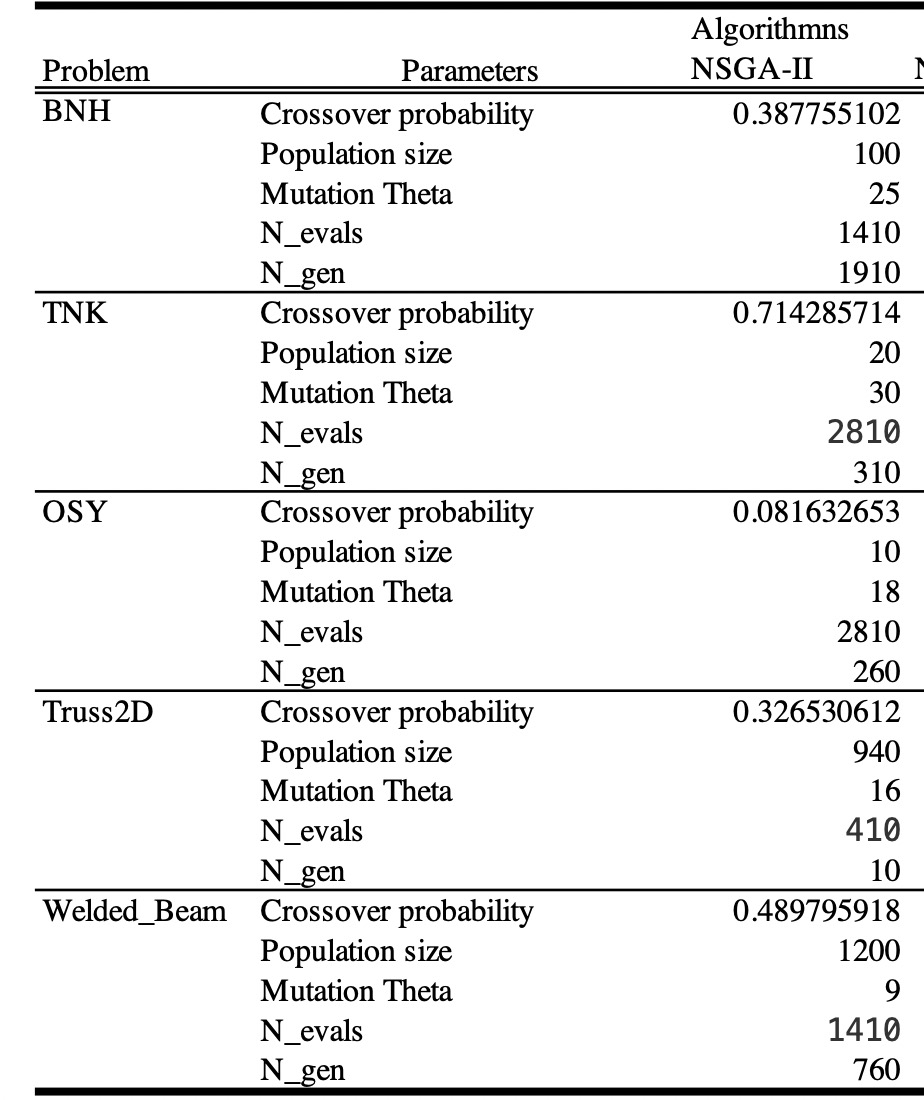
\includegraphics[width=6in, height = 14cm]{parameter_result.jpg}
\end{center}
\end{table}

\subsection{Outcome of algorithm files}
For different problems, algorithms files try to find various parameters. And then using parameters founded to process MOOP.

\section{Further Work}

\begin{itemize}
    \item For hypervolumn, calculating the Pareto front give data set
    \item From given Pareto front, calculating hypervolumn relative to some fixed points
    \item Studying two extra programs.
    \item To figure out NCI compile problem. 
\end{itemize} 

\section{Improvement}
The main problem of experiment is that I did not understand some algorithms very well. There may some potential 
errors in problem and algorithm files. Furthermore, not sure if I need to add visualization to each loop files.


\begin{center}
\bibliographystyle{plain}
\bibliography{report}
\end{center}

\end{document}


